\documentclass[a4paper, 11pt]{article}
\usepackage{comment} % enables the use of multi-line comments (\ifx \fi) 
\usepackage{lipsum} %This package just generates Lorem Ipsum filler text. 
\usepackage{fullpage} % changes the margin
\usepackage[a4paper, total={7in, 10in}]{geometry}
\usepackage[fleqn]{amsmath}
\usepackage{amssymb,amsthm}  % assumes amsmath package installed
\newtheorem{theorem}{Theorem}
\newtheorem{corollary}{Corollary}
\usepackage{graphicx}
\usepackage{tikz}
\usetikzlibrary{arrows}
\usepackage{verbatim}
\usepackage[numbered]{mcode}
\usepackage{float}
\usepackage{tikz}
    \usetikzlibrary{shapes,arrows}
    \usetikzlibrary{arrows,calc,positioning}

    \tikzset{
        block/.style = {draw, rectangle,
            minimum height=1cm,
            minimum width=1.5cm},
        input/.style = {coordinate,node distance=1cm},
        output/.style = {coordinate,node distance=4cm},
        arrow/.style={draw, -latex,node distance=2cm},
        pinstyle/.style = {pin edge={latex-, black,node distance=2cm}},
        sum/.style = {draw, circle, node distance=1cm},
    }
\usepackage{xcolor}
\usepackage{mdframed}
\usepackage[shortlabels]{enumitem}
\usepackage{indentfirst}
\usepackage{hyperref}
    
\renewcommand{\thesubsection}{\thesection.\alph{subsection}}

\newenvironment{problem}[2][Problem]
    { \begin{mdframed}[backgroundcolor=gray!20] \textbf{#1 #2} \\}
    {  \end{mdframed}}

% Define solution environment
\newenvironment{solution}
    {\textit{Solution:}}
    {}

\renewcommand{\qed}{\quad\qedsymbol}
%%%%%%%%%%%%%%%%%%%%%%%%%%%%%%%%%%%%%%%%%%%%%%%%%%%%%%%%%%%%%%%%%%%%%%%%%%%%%%%%%%%%%%%%%%%%%%%%%%%%%%%%%%%%%%%%%%%%%%%%%%%%%%%%%%%%%%%%
\begin{document}
%Header-Make sure you update this information!!!!
\noindent
%%%%%%%%%%%%%%%%%%%%%%%%%%%%%%%%%%%%%%%%%%%%%%%%%%%%%%%%%%%%%%%%%%%%%%%%%%%%%%%%%%%%%%%%%%%%%%%%%%%%%%%%%%%%%%%%%%%%%%%%%%%%%%%%%%%%%%%%
\large\textbf{Benjamin Smith} \hfill \textbf{Problem Set - 4}   \\
Email: bxs566@case.edu \hfill ID: 3559750 \\
\normalsize Course: CSDS 337 - Compiler Design \hfill Term: Spring 2024\\
Instructor: Dr. Vipin Chaudhary \hfill Due Date: $3^{rd}$ April, 2024 \\ \\
Number of hours delay for this Problem Set: \hfill 0\\
Cumulative number of hours delay so far: \hfill 40 \\ \\
I discussed this homework with: \hfill Jackson Schuetzle \\ \\
%\underline{\bf SUBMISSION GUIDELINES:} Submit a zip file that includes the %written answers and the flex file for Problem 4. \\

\noindent\rule{7in}{2.8pt}
%%%%%%%%%%%%%%%%%%%%%%%%%%%%%%%%%%%%%%%%%%%%%%%%%%%%%%%%%%%%%%%%%%%%%%%%%%%%%%%%%%%%%%%%%%%%%%%%%%%%%%%%%%%%%%%%%%%%%%%%%%%%%%%%%%%%%%%%
% Problem 1
%%%%%%%%%%%%%%%%%%%%%%%%%%%%%%%%%%%%%%%%%%%%%%%%%%%%%%%%%%%%%%%%%%%%%%%%%%%%%%%%%%%%%%%%%%%%%%%%%%%%%%%%%%%%%%%%%%%%%%%%%%%%%%%%%%%%%%%%
\begin{problem}{1 - 15 points}
Suppose that we have a production $A \rightarrow BCD$. Each of  the four nonterminals $A$ , $B$, $C$, and $D$ have two attributes: $s$ is a synthesized  attribute, and $i$ is an inherited attribute. For each of the sets of rules below,  tell whether (i) the rules are consistent with an S-attributed definition (ii) the  rules are consistent with an L-attributed definition, and (iii) whether the rules  are consistent with any evaluation order at all?  

\begin{enumerate}[a]
    \item $A.s = B.i + C.s.$  
    \item $A.s = B.i + C.s$ and $D.i = A.i + B.s.$  
    \item $A.s = B.s + D.s.$
    \item $A.s = D.i, \quad B.i = A.s + C.s, \quad C.i = B.s$, and $D.i = B.i + C.i.$ 
\end{enumerate}
    
\end{problem}
\begin{solution}

\begin{enumerate}[a]
    \item The rule is S-attributed. The rule is also L-attributed. The rule can be evaluated with a depth-first order.
    \item The rules are not S-attributed because $D.i$ is not in the head of the production and thus $D.i = A.i + B.s$ is an inherited attribute. The rules are L-attributed because there are no cyclic dependencies in the inherited attributes of $A$. The rules are consistent with a depth-first evaluation order.
    \item The rule is S-attributed and L-attributed. The rule is consistent with a depth-first evaluation order.
    \item The rules are not S-attributed. The rules are not L-attributed either because the rules $B.i = A.s + C.s$ and $C.i = B.s$ form a cyclic dependency. The rules are not consistent with any evaluation order because no acyclic dependency graph can be created for some inputs.
\end{enumerate}
\end{solution} 
\noindent\rule{7in}{2.8pt}

%%%%%%%%%%%%%%%%%%%%%%%%%%%%%%%%%%%%%%%%%%%%%%%%%%%%%%%%%%%%%%%%%%%%%%%%%
% Problem 2
%%%%%%%%%%%%%%%%%%%%%%%%%%%%%%%%%%%%%%%%%%%%%%%%%%%%%%%%%%%%%%%%%%%%%%%%%%%%%%%%%%%%%%%%%%%%%%%%%%%%%%%%%%%%%%%%%%%%%%%%%%%%%%%%%%%%%%%%

\begin{problem}{2 - 15 points}
Construct the DAG for the expression  $((x + y )-((x + y )* ( x - y ))) + ((x + y ) * ( x -  y ))$


\end{problem}
\begin{solution}

    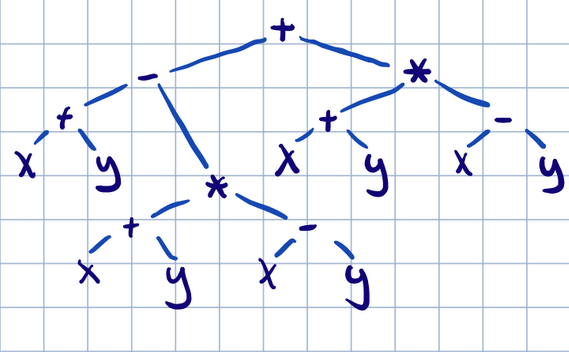
\includegraphics{DAG.png}

\end{solution} 
\noindent\rule{7in}{2.8pt}

%%%%%%%%%%%%%%%%%%%%%%%%%%%%%%%%%%%%%%%%%%%%%%%%%%%%%%%%%%%%%%%%%%%%%%%%%
% Problem 3
%%%%%%%%%%%%%%%%%%%%%%%%%%%%%%%%%%%%%%%%%%%%%%%%%%%%%%%%%%%%%%%%%%%%%%%%%%%%%%%%%%%%%%%%%%%%%%%%%%%%%%%%%%%%%%%%%%%%%%%%%%%%%%%%%%%%%%%%

\begin{problem}{3 - 15 points}
Translate the arithmetic expression $a + ( b + c )$. 

\begin{enumerate}[a]
    \item A syntax tree.  
    \item Quadruples. 
    \item Triples.  
    \item Indirect triples. 
\end{enumerate}
\end{problem}

\begin{solution}
\begin{enumerate}[a]
    \item  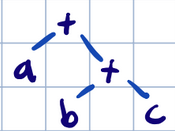
\includegraphics{AST.png}
    \item
        \begin{tabular}{|| c c c c c ||}
            \hline
            \# & Op & Arg1 & Arg2 & Res \\ [0.5ex]
            \hline\hline
            0 & + & b & c & t1 \\
            \hline
            1 & + & a & t1 & t2 \\
            \hline
        \end{tabular}
    \item
        \begin{tabular}{|| c c c c||}
            \hline
            \# & Op & Arg1 & Arg2 \\ [0.5ex]
            \hline\hline
            0  & +  & b    & c\\
            \hline
            1  & +  & a    & (0)\\
            \hline
        \end{tabular}
    \item 
        \begin{tabular}{|| c c||}
            \hline
            \# & Statement \\ [0.5ex]
            \hline\hline
            0  & (10)  \\
            \hline
            1  & (11)   \\
            \hline
        \end{tabular}
        \begin{tabular}{|| c c c c||}
            \hline
            \# & Op & Arg1 & Arg2 \\ [0.5ex]
            \hline\hline
            10  & +  & b    & c    \\
            \hline
            11  & +  & a    & (10)  \\
            \hline
        \end{tabular}
\end{enumerate}
\end{solution} 

\noindent\rule{7in}{2.8pt}
%%%%%%%%%%%%%%%%%%%%%%%%%%%%%%%%%%%%%%%%%%%%%%%%%%%%%%%%%%%%%%%%%%%%%%%%%
%%%%%%%%%%%%%%%%%%%%%%%%%%%%%%%%%%%%%%%%%%%%%%%%%%%%%%%%%%%%%%%%%%%%%%%%%
% Problem 4
%%%%%%%%%%%%%%%%%%%%%%%%%%%%%%%%%%%%%%%%%%%%%%%%%%%%%%%%%%%%%%%%%%%%%%%%%%%%%%%%%%%%%%%%%%%%%%%%%%%%%%%%%%%%%%%%%%%%%%%%%%%%%%%%%%%%%%%%

\begin{problem}{4 - 20 points}
A real array $A [i; j; k]$ has index $i$ ranging from 1 to 4, $j$  ranging from 0 to 4, and $k$ ranging from 5 to 10. Reals take 8 bytes each. If A  is stored row-major, starting at byte 0, find the location of:  

\begin{enumerate}[a]
    \item $A [3; 4 ; 5]$
    \item $A [1; 2 ; 7]$
    \item $A [4; 3 ; 9].$
\end{enumerate} 
Repeat the above if A is stored in column-major order.

\end{problem}

\begin{solution}

\noindent Row-major:
\begin{enumerate}[a]
    \item A row takes 5 * 4 * 8 = 160 bytes of space. The $i=3$ row starts at 320. Add 5 * 3 * 8 = 120 to get to the $j=4$ column in the row. Add 0 * 8 = 0 to get to the $k=5$ index in the column. The location of $A[3;4;5]$ is at 440 bytes.
    \item 40 + 16 = 56 bytes.
    \item 480 + 80 + 72 = 632 bytes.
\end{enumerate} 
Column-major:
\begin{enumerate}[a]
    \item 
    \item 
    \item 
\end{enumerate} 

\end{solution} 

%%%%%%%%%%%%%%%%%%%%%%%%%%%%%%%%%%%%%%%%%%%%%%%%%%%%%%%%%%%%%%%%%%%%%%%%%
%%%%%%%%%%%%%%%%%%%%%%%%%%%%%%%%%%%%%%%%%%%%%%%%%%%%%%%%%%%%%%%%%%%%%%%%%
% Problem 5
%%%%%%%%%%%%%%%%%%%%%%%%%%%%%%%%%%%%%%%%%%%%%%%%%%%%%%%%%%%%%%%%%%%%%%%%%%%%%%%%%%%%%%%%%%%%%%%%%%%%%%%%%%%%%%%%%%%%%%%%%%%%%%%%%%%%%%%%

\begin{problem}{5 - 20 points}
Add rules to the syntax-directed definition of Fig. ~\ref{fig_5}  for  the following control-flow constructs:  
\begin{figure}[H]
    \centering
    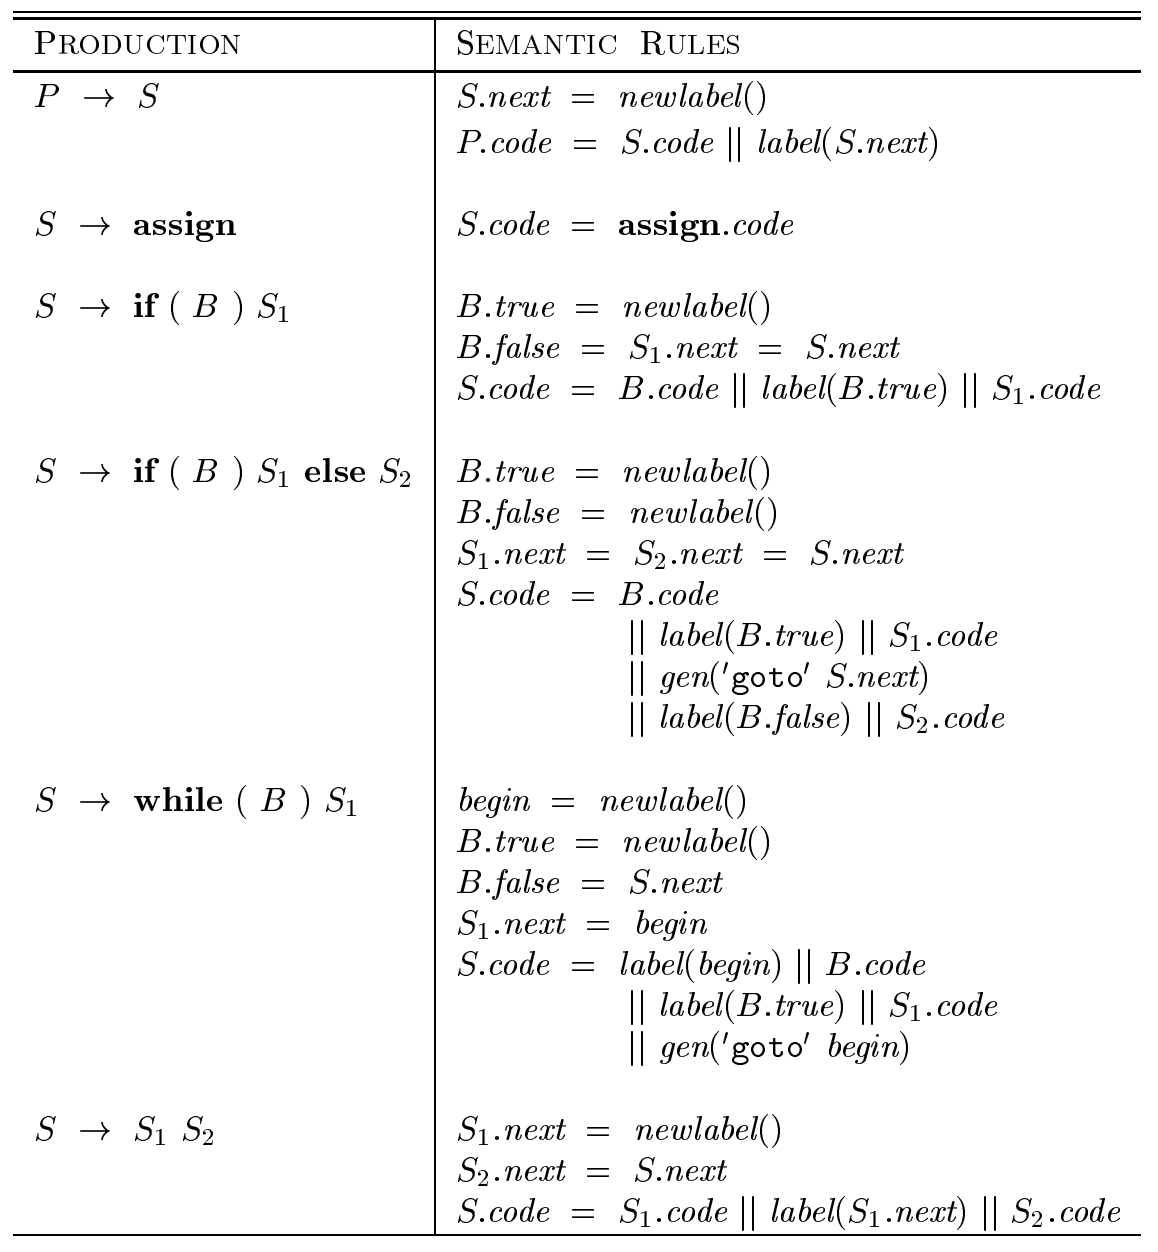
\includegraphics[scale=0.75]{sdd.png}
    \caption{Rules to the syntax-directed definition}
    \label{fig_5}
\end{figure}

\begin{itemize}
    \item A repeat-statement {\bf repeat} $S$ {\bf while} $B$.
    \item A for-loop {\bf for} $(S_1; B ; S_2 ) S_3$. 
\end{itemize}

\end{problem}

\begin{solution}
    $S \rightarrow$ {\bf for} $(S_1; B; S_2) S_3$ \\
    $begin = newlabel() \\
    B.true = newlabel() \\
    B.false = S.next \\
    S_3.next = begin \\
    S.code = S_1.code \quad || \quad label(begin) \quad || \quad B.code \\
    || \quad label(B.true) \quad || \quad S_3.code \quad || \quad S_2.code \\
    || \quad gen(\text{'goto' } begin)$
\end{solution} 

%%%%%%%%%%%%%%%%%%%%%%%%%%%%%%%%%%%%%%%%%%%%%%%%%%%%%%%%%%%%%%%%%%%%%%%%%
%%%%%%%%%%%%%%%%%%%%%%%%%%%%%%%%%%%%%%%%%%%%%%%%%%%%%%%%%%%%%%%%%%%%%%%%%
% Problem 6
%%%%%%%%%%%%%%%%%%%%%%%%%%%%%%%%%%%%%%%%%%%%%%%%%%%%%%%%%%%%%%%%%%%%%%%%%%%%%%%%%%%%%%%%%%%%%%%%%%%%%%%%%%%%%%%%%%%%%%%%%%%%%%%%%%%%%%%%

\begin{problem}{6 - 15 points}
Translate the following expressions using the ifFalse mechanism: 

\begin{enumerate}[a]
    \item if $(a==b \quad \&\& \quad c==d \quad || \quad e==f) \quad x = 1$;  
    \item if $(a==b \quad || \quad c==d \quad || \quad e==f) \quad x = 1$;  
    \item if $(a==b \quad \&\& \quad c==d \quad \&\& \quad e==f) \quad x = 1$; 
\end{enumerate}

\end{problem}

\begin{solution}
\begin{enumerate}[a]
    \item ifFalse $(a  != b \quad || \quad c != d \quad \&\& \quad e != f) \quad x = 1;$
    \item ifFalse $(a  != b \quad \&\& \quad c != d \quad \&\& \quad e != f) \quad x = 1;$
    \item ifFalse $(a  != b \quad || \quad c != d \quad || \quad e != f) \quad x = 1;$
\end{enumerate}
\end{solution} 

%%%%%%%%%%%%%%%%%%%%%%%%%%%%%%%%%%%%%%%%%%%%%%%%%%%%%%%%%%%%%%%%%%%%%%%%%
%%%%%%%%%%%%%%%%%%%%%%%%%%%%%%%%%%%%%%%%%%%%%%%%%%%%%%%%%%%%%%%%%%%%%%%%%
% Problem 7
%%%%%%%%%%%%%%%%%%%%%%%%%%%%%%%%%%%%%%%%%%%%%%%%%%%%%%%%%%%%%%%%%%%%%%%%%%%%%%%%%%%%%%%%%%%%%%%%%%%%%%%%%%%%%%%%%%%%%%%%%%%%%%%%%%%%%%%%


\noindent\rule{7in}{2.8pt}

\end{document}
 